\chapter{The Cross-Layer Approach and the DPU Substrate}
\label{ch:background}

In 2010, a group of researchers eavesdropped on a commercial QKD link and read
the secret key in full, without leaving a trace
in the error rate that was supposed to expose them. 
They did not exploit a fault in the photonic devices, nor did they find a vulnerability in the
QKD protocol. 
Instead, they shone a continuous beam of bright light
into the receiver, driving its single-photon detectors out of their quantum
regime and into a classical mode in which they responded only to a sharp spike of
power. From that point on, the attacker could decide exactly when each detector
``clicked'' and thereby dictate the key the two endpoints believed they had shared
in secret~\cite{lydersen2010hacking}.
The mathematics was untouched and the hardware behaved exactly as it was built to.
The weakness lived in the seam between them: a silent assumption the protocol layer
made about the device layer---that a single-photon detector responds to light the
way its idealized model says it does. Examined on its own terms, neither layer was
at fault. The vulnerability existed only at their boundary, where one layer's proof
met the other's physics.

This episode is a small parable for the argument of this dissertation. The
exploitable weakness belonged to no single layer; it emerged where they met, at an
interface whose assumptions no one had thought to test. A guarantee established at
one layer of a secure system is only as strong as what it takes for granted about
the layers above and below it---and it is at those boundaries, rather than within
any one layer, that security tends to fail. The paper-centric chapters that follow span photonic devices, quantum-key
post-processing, post-quantum cryptographic acceleration, datacenter transport,
and security observability. Read individually, they appear to belong to separate
research communities, each with its own models, metrics, and implicit assumptions.
Two things make them a single dissertation: a shared \emph{method}---a cross-layer
view of secure communication in which a design choice at one layer is judged by its
consequences at the others---and a shared \emph{substrate}---the data processing
unit (DPU) on which nearly every contribution is built or observed.

This chapter establishes only those two common threads. It first sets out the
cross-layer lens and the analytical method that recur throughout the thesis, and
then introduces the DPU as the hardware that connects cryptographic primitives to
the infrastructure. The technical background specific to each topic---integrated
photonic sources, QKD post-processing, post-quantum primitives, RDMA fabrics, and
confidential computing---is deliberately deferred to the chapter that needs it,
where it can be developed alongside the corresponding contribution. The cross-layer
dependencies that emerge once all of these pieces are in place are revisited and
resolved in Chapter~\ref{ch:cross-layer}.

\section{The Cross-Layer Security Stack}
\label{sec:bg-stack}

The introduction framed the quantum threat not merely as an algorithm-selection
problem, but as a systemic architectural challenge governed by the boundaries
between the device, protocol, and infrastructure layers. Information value decay
explains \emph{which} protection each class of traffic warrants rather than why the
problem is cross-layer: unconditionally high-value, slowly decaying secrets justify
the deployment complexity and bespoke hardware of physics-based security, primarily
QKD, which offers information-theoretic security that is immune to algorithmic
advances, while the much larger volume of computationally protected, rapidly
decaying traffic is served by PQC, which must operate at datacenter scale. What
makes the problem cross-layer is that both physics-based and computationally-based
protections must ultimately run on the same programmable network fabric, where
their device- and protocol-level guarantees collide with one shared set of
infrastructure constraints.

To analyze this heterogeneous landscape, this dissertation structures the response
along three distinct but interacting layers, illustrated in Figure~\ref{fig:cross_layer_stack}.

\begin{figure}[htbp]
    \centering
    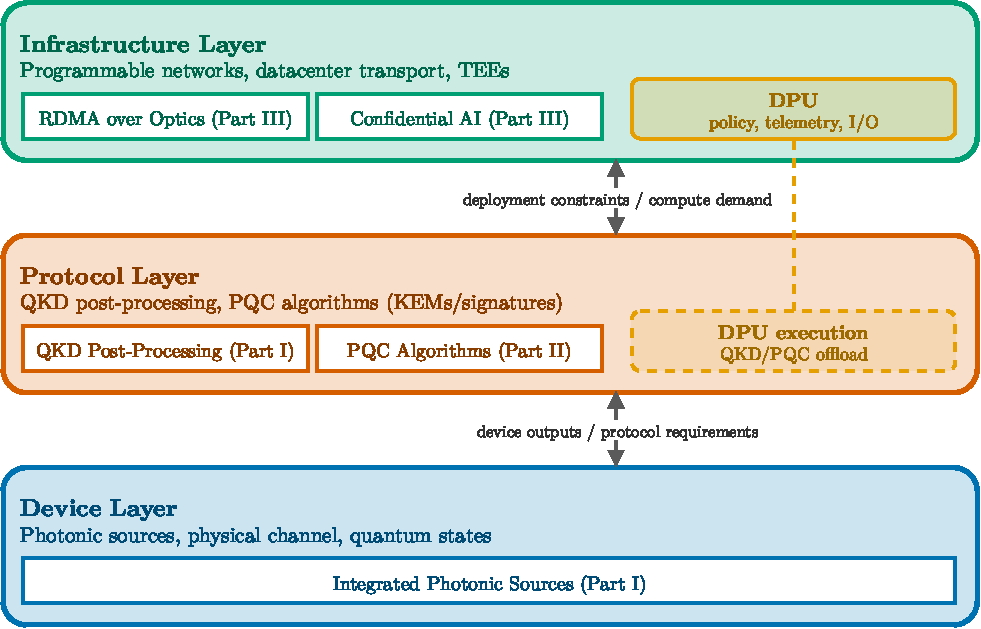
\includegraphics[width=0.85\textwidth]{figures/chapter2/cross_layer_stack.pdf}
    \caption{The cross-layer security stack investigated in this dissertation. The device layer supplies physical resources; the protocol layer consumes those resources to produce key material and authenticated channels; the infrastructure layer determines deployment viability. The Data Processing Unit (DPU) serves as both the execution substrate and observation point spanning the upper layers.}
    \label{fig:cross_layer_stack}
\end{figure}

\begin{itemize}
  \item a \textbf{device layer}, where photonic sources and the physical channel
        determine the quality and stability of the quantum states that security
        protocols can assume. The governing quantities here are physical: spectral
        purity, free spectral range (FSR), quality factors, and loss budgets.
  \item a \textbf{protocol layer}, where QKD post-processing and post-quantum
        algorithms turn raw physical or mathematical resources into usable key
        material and authenticated channels. The governing quantities here are
        algorithmic and informational: key distillation rates, security margins,
        computational complexity, and message sizes.
  \item an \textbf{infrastructure layer}, where programmable network hardware,
        datacenter transport, and confidential-computing environments decide
        whether those protocols can actually be deployed, accelerated, observed,
        and defended at scale. The governing quantities here are operational:
        latency, throughput, determinism, queue depth, and observability.
\end{itemize}

\subsection{The Cross-Layer Method}

The recurring method of the thesis is to take a security or performance
assumption stated at one layer and test what happens to it when it is mapped
onto another. An isolationist view often hides systemic vulnerabilities. For
instance, a protocol proof might assume perfect single-photon sources, while the
device layer actually exposes multiphoton states subject to thermal drift. A
post-quantum signature scheme might be highly efficient when benchmarked on a
single idle core, but its tail latency might collapse under heavy datacenter
batching. A transport layer might be provably encrypted by MACsec or IPsec, yet
still leak critical application state through traffic ordering and timing behavior.
Finally, an infrastructure defender operating a confidential-computing cluster must
detect intrusions without seeing the payload, violating the assumptions of classical
intrusion detection systems.

Research questions RQ1--RQ3 each target a single layer---PQC deployment, QKD
architecture, and photonic-source design---while RQ4 binds them by exposing
exactly these cross-layer failure modes.

\section{Programmable Network Infrastructure for Security Offload}
\label{sec:bg-dpu}

The single piece of hardware common to nearly every contribution in this thesis is
the DPU. It is introduced here, once, because it underpins the QKD, PQC, and
infrastructure chapters alike.

SmartNICs and DPUs represent a paradigm shift in datacenter architecture. They extend
the network interface from a passive I/O endpoint---responsible only for moving packets
between the wire and host memory---into an active, programmable execution environment.
In modern DPU architectures like the NVIDIA BlueField series, the device features a
cluster of general-purpose Arm CPU cores, dedicated hardware accelerators (including
inline cryptographic engines for AES-GCM and public-key acceleration), substantial
on-board memory, and programmable packet-processing pipelines~\cite{burstein2021nvidia}.
In more advanced configurations, DPUs provide direct GPU-connected datapaths (e.g.,
GPUDirect remote direct memory access, RDMA) that bypass the host CPU entirely
(Figure~\ref{fig:dpu_architecture}).

\begin{figure}[htbp]
    \centering
    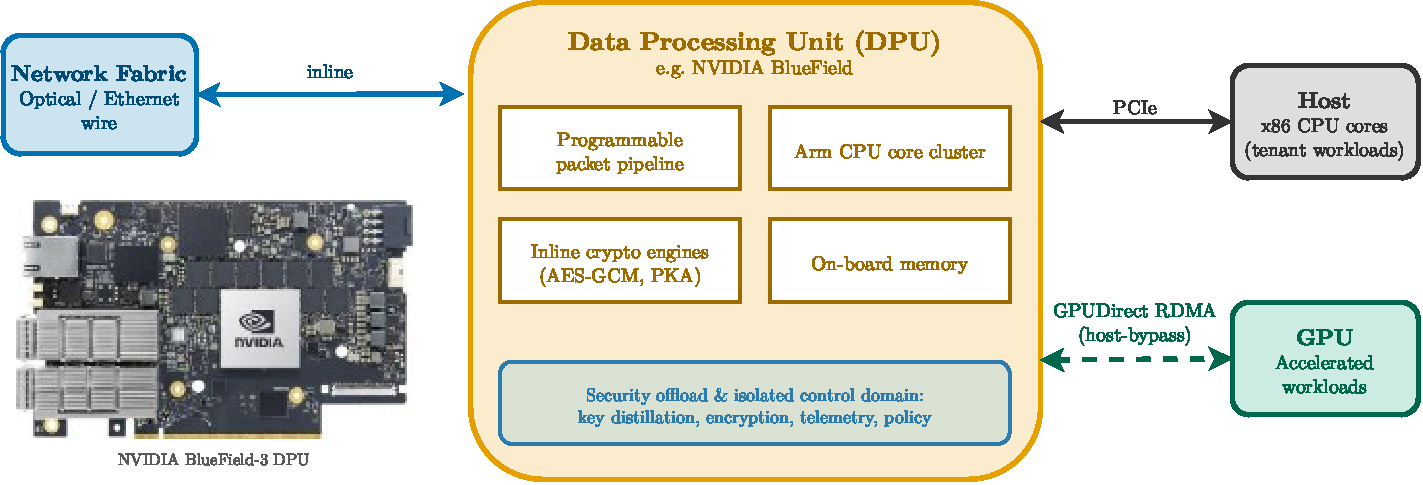
\includegraphics[width=0.95\textwidth]{figures/chapter2/dpu_architecture.pdf}
    \caption{The DPU as an execution substrate and observation point. Sitting
    inline between the network fabric and the host, the DPU couples a programmable
    packet pipeline, an Arm CPU core cluster, inline cryptographic engines, and
    on-board memory. Security-critical functions are offloaded into this isolated
    control domain, while a GPUDirect RDMA datapath moves data to the GPU without
    traversing the host CPU.}
    \label{fig:dpu_architecture}
\end{figure}

This architecture makes it possible to place security-critical operations---such as
key distillation, cryptographic encapsulation, storage encryption, telemetry collection,
and firewall policy enforcement---at the edge of the host rather than deep inside its
operating system~\cite{meyer2026hqc}. By moving these functions to the DPU, the host CPU
is freed to run tenant workloads, and the infrastructure provider retains a secure,
isolated domain to enforce policies even if the host is compromised.

\subsection{The Offload Decision Framework}

However, offload is not automatically beneficial. Moving a task from a powerful,
high-frequency x86 host CPU to a lower-power Arm core on a DPU introduces significant
overheads: data movement across the PCIe bus, queueing delays, synchronization locks,
resource contention among DPU cores, and additional software complexity. The host CPU
will almost always win a raw single-thread benchmark.

Therefore, the useful question is never whether a DPU is ``faster'' in isolation. The
relevant architectural questions are:
\begin{enumerate}
    \item \textbf{Partitioning:} Which specific part of a pipeline should move to the DPU?
    \item \textbf{Batching:} Under what traffic conditions and batch sizes does the offload break even?
    \item \textbf{Bottlenecks:} What becomes the new system bottleneck once the compute task has moved?
    \item \textbf{Determinism:} How stable is the latency distribution under heavy, concurrent load?
\end{enumerate}

These questions recur in identical form across different domains in this thesis. They
dictate how QKD post-processing scales (Chapter~\ref{ch:qkd-dpu}), whether post-quantum
key encapsulation meets handshake latency budgets (Chapter~\ref{ch:dpu-pqc}), and how
secured end-to-end AI pipelines manage image I/O (Chapter~\ref{ch:ai-pipelines}). For this reason,
the DPU is treated here as a unifying substrate rather than as a detail of any single
chapter.

Furthermore, the same programmability that enables offload also transforms the DPU into
a natural observation point. Placed inline between the network and the host, the DPU
can inspect traffic metadata, connection timing, and queue depths without host interference,
a capability that becomes the foundation of the confidential-AI observability discussed
in Chapter~\ref{ch:confidential-ai}.
